% !TeX root = mos-en.tex

%%%%%%%%%%%%%%%%%%%%%%%%%%%%%%%%%%%%%%%%%%%%%%%%%%%%%%%%%%%%%%%%

\begin{prob}{Birthday pairings}
Randomly select $23$ people and ask them what their birthdays are. Assume a uniform distribution of $365$ different birthdays (no one was born on February $29$). Show that the probability that at least two of them have the same birthday is greater than $0.5$.
\end{prob}

\solution{}

Compute the probability that none of the $23$ people have the same birthday and show that it is less than $0.5$. Select the first birthday arbitrarily, then the next birthday from the remaining days, then the next birthday from the remaining days, and so on:
\[
\renewcommand*{\arraystretch}{2.5}
\begin{array}{rcl}
P(\textsf{no birthday pair})&=&
  \overbrace{\disfrac{365}{365}\cdot\frac{364}{365}
  \cdot\frac{363}{365}\cdot \;\cdots \; \cdot \frac{344}{365}
  \cdot\frac{343}{365}}^{23\;\textsf{\small fractions}}\\
&=&\disfrac{365!}{365^{23}\cdot 342!}\approx 0.4927\,.
\end{array}
\]
Most people guess that more than $23$ people are needed to find two with the same birthday!

A modern calculator can compute the probability, but it is worthwhile computing it using Stirling's approximation $\ln n! \approx n\ln n - n$:
\[
\renewcommand*{\arraystretch}{2}
\begin{array}{rcl}
\ln P(\textsf{no birthday pair})&=&
  \ln\left(\disfrac{365!}{342!\cdot 365^{23}}\right)=\ln 365! - \ln 342! -23 \ln 365\\
&\approx& (365\ln 365 -365) - (342\ln 342 -342) - 23\,\ln 365 \\
&\approx&-0.7404\\
P(\textsf{no birthday pair})&\approx&e^{-0.7404}=0.4769\,.
\end{array}
\]
The reader is invited to compute the probability with the following better approximation:
\[
\ln n!  \approx n\ln n - n + \frac{1}{6}\left(8n^3+4n^2+n+\frac{1}{30}\right)+\frac{1}{2}\ln\pi\,.
\]
\textbf{Simulation}
\begin{verbatim}
For 21 people:
Expectation of no pairs = 0.5563
Average no pairs        = 0.5497
For 22 people:
Expectation of no pairs = 0.5243
Average no pairs        = 0.5237
For 23 people:
Expectation of no pairs = 0.4927
Average no pairs        = 0.4933
For 24 people:
Expectation of no pairs = 0.4617
Average no pairs        = 0.4576
For 25 people:
Expectation of no pairs = 0.4313
Average no pairs        = 0.4345
\end{verbatim}

%%%%%%%%%%%%%%%%%%%%%%%%%%%%%%%%%%%%%%%%%%%%%%%%%%%%%%%%%%%%%

\begin{prob}{Finding your birthmate}
Your \emph{birthmate} is a person with the same birthday as yours.

Why is finding a birthmate a different problem than finding a birthday pairing?

\que{1} How many people do you have to ask until the probability of finding your brithmate becomes greater than $0.5$?

\que{2}
Solve the problem by using the approximation in Equation~\ref{eq.reciprocal} (page~\pageref{eq.reciprocal}).
\end{prob}

\solution{}

Many people could have the same birthday which is considered a success for find a birthday pairing, but not for finding a birthmate unless that birthday is the same as yours.

\ans{1}
Find the smallest number of people for which the probability that none of them are birthmates is less than $0.5$. The probability that the first person you ask is not a birthmate is $364/365$, but that is also the probability that the second, third, \ldots, person is not a birthmate. The solution is the smallest $k$ such that:
\[
P(\textsf{birthmate not found})=\left(\frac{364}{365}\right)^k<\frac{1}{2}\,,
\]
which is $k=253$:
\[
\left(\frac{364}{365}\right)^{253} \approx 0.4995\,.
\]
\ans{2}
Equation~\ref{eq.reciprocal} is:
\[
\lim_{n\rightarrow\infty}\left(\frac{n-1}{n}\right)^{n}=\frac{1}{e}\,,
\]
which can be used to approximate the probability:
\begin{eqn}
P(\textsf{birthmate not found})&=&
  \left(\disfrac{365-1}{365}\right)^k=\left[\left(\disfrac{364}{365}\right)^{365}\right]^{k/365}\\
&\approx& e^{-k/365}\\
e^{-253/365}&\approx&0.5000\,.
\end{eqn}
\textbf{Simulation}
\begin{verbatim}
For 251 people:
Probability of no match = 0.5023
Proportion no match     = 0.5120
For 252 people:
Probability of no match = 0.5009
Proportion no match     = 0.5055
For 253 people:
Probability of no match = 0.4995
Proportion no match     = 0.4984
For 254 people:
Probability of no match = 0.4982
Proportion no match     = 0.4987
For 255 people:
Probability of no match = 0.4968
Proportion no match     = 0.5078
\end{verbatim}


%%%%%%%%%%%%%%%%%%%%%%%%%%%%%%%%%%%%%%%%%%%%%%%%%%%%%%%%%%%%%

\begin{prob}{Relating the birthday pairings and the birthmate problems}
Let $P_{\textsf{\footnotesize pair}}(r)$ be the probability that out of $r$ people two are a birthday pair (Problem~$31$) and let $P_{\textsf{\footnotesize mate}}(n)$ be the probability that out of $n$ people at least one is your birthmate (Problem~$32$). Given $r$, for what $n$ does $P_{\textsf{\footnotesize pair}}(r) \approx P_{\textsf{\footnotesize mate}}(n)$?
\end{prob}

\solution{1}

The solution is based on \cite{birthday}.

Using the notation $P_{\textsf{\footnotesize no pair}}(r)$ for the complement of $P_{\textsf{\footnotesize pair}}(r)$, from the solution to Problem~$31$ we have:
\[
\renewcommand*{\arraystretch}{2.2}
\begin{array}{lcl}
P_{\textsf{\footnotesize no pair}}(r)&=&
\disfrac{365}{365}\cdot 
  \frac{365-1}{365}\cdot \frac{365-2}{365} \cdot\;
  \cdots \;\cdot \frac{365-(r-1)}{365}\\
&=&1\left(1-\disfrac{1}{365}\right)
  \left(1-\disfrac{2}{365}\right) \cdot\;
  \cdots \;\cdot \left(1-\disfrac{r-1}{365}\right)\\
&\approx&1-\disfrac{1}{365} - \disfrac{2}{365} -
  \cdots - \disfrac{r-1}{365}\\
&=&1-\disfrac{1+2+3+\cdots + (r-1)}{365}\\
&=&1-\disfrac{r(r-1)/2}{365}\,,
\end{array}
\]
where the approximation in the third equation results from deleting powers of $1/365$ greater than one because they are too small to significantly affect the result.

Using the notation $P_{\textsf{\footnotesize no mate}}(n)$ for the complement and the same approximation, from the solution to Problem~$32$ we have:
\[
\renewcommand*{\arraystretch}{2.2}
\begin{array}{lcl}
P_{\textsf{\footnotesize no mate}}(n)
&=&\overbrace{\left(1-\frac{1}{365}\right)
  \left(1-\frac{1}{365}\right)\cdots
  \left(1-\frac{1}{365}\right)}^{n}\\
&\approx& 1-\overbrace{\frac{1}{365}-\frac{1}{365}\cdots-
  \frac{1}{365}}^{n}\\
&\approx& 1-\disfrac{n}{365}\\
\end{array}
\]
Therefore $P_{\textsf{\footnotesize no pair}}(r)\approx P_{\textsf{\footnotesize no mate}}(n)$ when:
\[
n=\frac{r(r-1)}{2}\,.
\]
For $r=23$, $n=(23\cdot 22)/2=253$.

\solution{2}

Mosteller \cite[p.~322]{birthday} gives the following intuitive solution:
\begin{quote}
In comparing the birthday and birthmate problems, one observes that for $r$ people in the birthday problem, there are $r(r-1)/2$ pairs or \emph{opportunities} for like birthdays; whereas, if $n$ people are questioned in the birthmate problem, there are only $n$ opportunities for me to find one or more birthmates.
\end{quote}
From this he concludes that $n\approx r(r-1)/2$.

This reasoning can be understood as follows: For the birthday problem choose an arbitrary date and ask if two people out of $r$ have \emph{that birthday}. There are:
\[
{r \choose 2}=\frac{r!}{2!(r-2)!} = \frac{r(r-1)}{2}
\]
ways of doing so. For the birthmate problem your own birthday is given. Any of the $n$ people can have the same birthday. By equating the two expressions we have the $n$ such that $P_{\textsf{\footnotesize pair}}(r) \approx P_{\textsf{\footnotesize mate}}(n)$.

\textbf{Simulation}

You can run the simulations using the programs for Problems~31, 32 and check this result.

%%%%%%%%%%%%%%%%%%%%%%%%%%%%%%%%%%%%%%%%%%%%%%%%%%%%%%%%%%%%%

\begin{prob}{Birthday holidays\annotate{D}}
A factory is closed whenever one of its workers has a birthday. There are no other holidays.

\que{1} How many workers should be employed in order to maximize the number of work-days in one year?

\que{2} What is the expectation of the ratio of the maximum work-days to $365^2$, the number of possible work-days if each one of $365$ workers worked every day?

\textbf{Hint:} Prove that there must be a maximum by considering extreme cases. Then develop a formula for the expectation of the number of work-days for a single day.
\end{prob}

\solution{}

\ans{1}
At one extreme if there is only one worker there are $364$ work-days. If there are two workers there are $363+363=726$ workers days (ignoring the very small possibility that both workers have the same birthday). At the other extreme if there are one million workers the number of work-days will almost certainly be zero. Since the number of work-days rises initially and then returns to zero, there must be a maximum in between the extremes.

To simplify the notation we will denote the number of days in a year by $N$ and the number of workers by $n$.

For any given day the probability that it is a work-day is the probability that each worker has a birthday on some other day:
\[
P(\textsf{a given day is a work-day})=\overbrace{\disfrac{N-1}{N} \cdot \;\cdots\;\cdot \disfrac{N-1}{N}}^n = \left(1-\disfrac{1}{N}\right)^n\,.
\]
Denote $\left(1-\disfrac{1}{N}\right)$ by $p$. Then:
\[
E(\textsf{work-days for a given day}) = n \cdot p^n + 0\cdot (1-p^n) = np^n\,.
\]
All the days in the year have this same expectation, so we just multiply by $N$ to get the expectation for a year:
\begin{equation}\label{eq.holidays}
E(\textsf{work-days for a year}) = Nnp^n\,.
\end{equation}

To find the maximum we take the derivative of Equation~\ref{eq.holidays} with respect to $n$ and use $(p^n)'=p^n\ln p$ which can be proved using the chain rule:
\[
(p^n)' = ((e^{\ln p})^n)' =
(e^{n\ln p})' =
e^{n\ln p} (n\ln p)'=
(e^{\ln p})^n \ln p = p^n\ln p\,.
\]
The derivative of Equation~\ref{eq.holidays} is therefore:
\[
(Nnp^n)'= N (p^n + n (p^n)') = N (p^n + np^n\ln p)\,,
\]
which is $0$ when:
\[
n=-\disfrac{1}{\ln p}\,.
\]
For $N=365$ this gives $n=364.5$. Since $n$ is a positive integer the maximum is achieved at $n=364$ or $n=365$ which give the same expectation of the number of work-days:
\begin{eqn}
E(\textsf{work-days for a year}) &=&Nnp^n\\
&=&365\cdot 364 \cdot \left(\disfrac{364}{365}\right)^{364}\\
&=&365\cdot 364  \cdot \disfrac{365}{365}\left(\disfrac{364}{365}\right)^{364}\\
&=&365\cdot 365  \cdot \left(\disfrac{364}{365}\right)^{365}\\
&=&48944\,.
\end{eqn}

\ans{2} 
The expectation of the ratio is:
\[
E(\textsf{max work-days/possible work-days})=\disfrac{365\cdot 365  \cdot \left(\frac{364}{365}\right)^{365}}{365\cdot 365}=\left(\disfrac{364}{365}\right)^{365}\approx 0.3674\,.
\]
By Equation~\ref{eq.reciprocal}:
\[
\lim_{n\rightarrow\infty}E(\textsf{max work-days/possible work-days})=\lim_{N\rightarrow \infty} \left(1-\disfrac{1}{N}\right)= \disfrac{1}{e}\,.
\]

\textbf{Simulation}
\begin{verbatim}
For 100 people
Expectation work-days    = 27742
Average work days        = 27743
Ratio work-days / 365**2 = 0.2082
For 250 people
Expectation work-days    = 45958
Average work days        = 45939
Ratio work-days / 365**2 = 0.3450
For 364 people
Expectation work-days    = 48944
Average work days        = 48936
Ratio work-days / 365**2 = 0.3674
For 365 people
Expectation work-days    = 48944
Average work days        = 48917
Ratio work-days / 365**2 = 0.3674
\end{verbatim}

%%%%%%%%%%%%%%%%%%%%%%%%%%%%%%%%%%%%%%%%%%%%%%%%%%%%%%%%%%%%%

\begin{prob}{The cliff-hanger}
A particle is initially placed on the $x$-axis at position $1$. At any position on the $x$-axis it can move right with probability $2/3$ and left with probability $1/3$ (Figure~\ref{f.ruin1}).

\que{1} What is the probability that the particle will eventually be at position $0$?

\que{2} If the probability of moving right is $p$ and the probability of moving left is $1-p$, what is the probability that the particle will eventually be at position $0$? Analyze the result for various values of $p$.

\textbf{Hint:} Use conditional probabilities after the first move.
\begin{figure}[tb]
\begin{center}
\begin{tikzpicture}[scale=1.5]
\draw (0,0) -- (6,0);
\draw[dashed] (6,0) -- (8,0) node[right] {$\infty$};
\foreach \x in {0,1,2,3,4,5,6} {
  \draw (\x,0) -- +(0,4pt);
  \node at (\x,-10pt) { $\x$ };
}
\draw[fill] (1,5mm) circle[radius=.5pt];
\draw[->] (1,5mm) -- node[above] {$1/3$} (0,5mm);
\draw[->,very thick] (1,5mm) -- node[above] {$2/3$} (2,5mm);

\foreach \x/\y in {2/10mm,3/15mm,4/20mm} {
  \draw[fill] (\x,\y) circle[radius=.5pt];
  \draw[->] (\x,\y) -- node[above] {$1/3$} (\x-1,\y);
  \draw[->] (\x,\y) -- node[above] {$2/3$} (\x+1,\y);
}
\end{tikzpicture}
\end{center}
\caption{Can the particle return to $0$ (axis is infinite to the right)?}\label{f.ruin1}
\end{figure}
\end{prob}

\solution{}

It is no more difficult to compute the probabilty for arbitrary $p$ as it is for $p=2/3$, so we give solutions for both questions together.

\ans{1,2}
Let us try to compute the probability directly. Denote a move left by $L$ and a move right by $R$. The particle can reach $0$ directly by moving $L$ with probability $\frac{1}{3}$, or by moving $RLL$ with probability $\frac{2}{3}\cdot\frac{1}{3}\cdot\frac{1}{3}$, or by moving $RRLLL$ with probability $\left(\frac{2}{3}\right)^2\left(\frac{1}{3}\right)^3$, \ldots\ . This computations seems to be a straightforward geometric progression, but it ignores possibilities such as $RLRLL$.

Compute the probability that the particle reaches $0$ from $1$ conditioned on the first step:
\begin{eqn}
P(\textsf{reaches}\;0\;\textsf{from}\;1) &=& P(\textsf{reaches}\;0\;\textsf{from}\;1|\textsf{first move left}) +\\
&&P(\textsf{reaches}\;0\;\textsf{from}\;1|\textsf{first move right})\\
&=& (1-p)\cdot 1 + pP(\textsf{reaches}\;1\;\textsf{from}\;2)P(\textsf{reaches}\;0\;\textsf{from}\;1)\,.
\end{eqn}
But the probability of reaching $1$ from $2$ is exactly the same as the probability of reaching $0$ from $1$. Denoting $P(\textsf{reaches}\;0\;\textsf{from}\;1)$ by $P$ we have:
\begin{eqn}
P &=& (1-p) + pP^2\\
pP^2 - P + (1-p) &=&0\\
P&=& \frac{1\pm\sqrt{1-4p(1-p)}}{2p}\\
P&=&1,\; (1-p)/p\,.
\end{eqn}
If $p\leq 1/2$ then $(1-p)/p\geq 1$, so $P=1$ is the only solution and it is certain that the particle will reach $0$.

If $p=1$ then $P=0$ since if the particle always moves to the right it cannot return to $0$.

Suppose $P=1$ for $1/2<p < 1$, that is, $P$ \emph{does not depend on} $p$. But $P$ cannot suddenly ``jump'' from $1$ to $0$ as $p$ approaches $1$: in Figure~\ref{f.ruin2} the dashed red line and the red dot at $(1,0)$. Therefore, for $p> 1/2$ the only solution is $P=(1-p)/p< 1$.\footnote{Mosteller writes that this follows by continuity but does not give a proof.}

\begin{figure}[tb]
\begin{center}
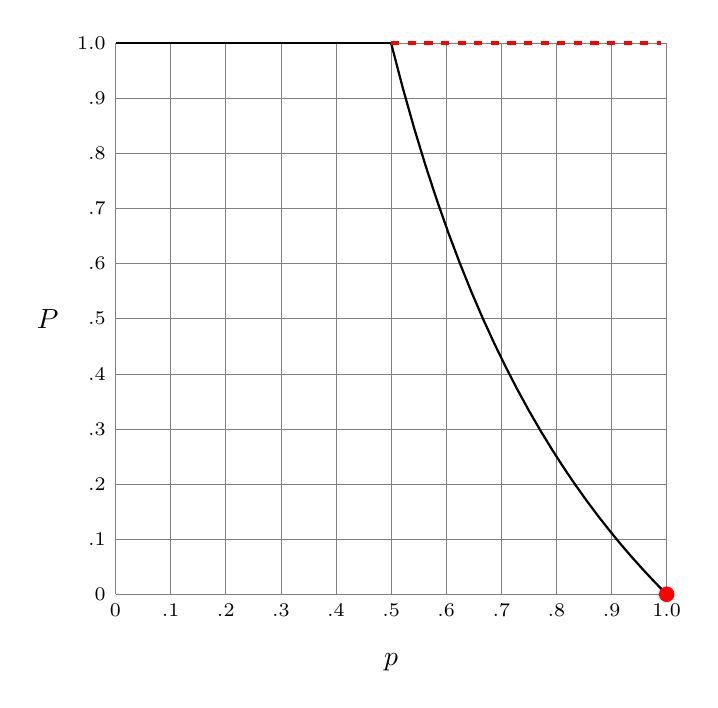
\begin{tikzpicture}[scale=7]
\draw[help lines,step=.1] (0,0) grid (1,1);
\foreach \x in {0,.1,.2,.3,.4,.5,.6,.7,.8,.9,1.0}
  \node[below] at (\x,0) {$\scriptstyle \x$};
\foreach \y in {0,.1,.2,.3,.4,.5,.6,.7,.8,.9,1.0}
  \node[left] at (0,\y) {$\scriptstyle \y$};
\draw[domain=0:.5,thick] plot (\x,1);
\draw[domain=.5:1,thick] plot (\x,{(1-\x)/\x});
\node at (.5,-3.5pt) {$p$};
\node at (-3.5pt,.5) {$P$};
\draw[ultra thick,red,dashed] (.5,1) -- +(.49,0);
\fill[red] (1,0) circle[radius=.4pt];
\end{tikzpicture}
\end{center}
\caption{Graph of $P=\min(p/(1-p),1)$ for $p\in [0,1]$}\label{f.ruin2}
\end{figure}
For $p=2/3, P=1/2$ and for $p=1/2, P=1$. This is a surprising result because one would not expect that the particle would always return to $0$ if the direction of the moves were determined by flipping a fair coin! You have to have a very unfair coin (probability of heads is $2/3$) to even the chances or returning to $0$ or not.

\textbf{Simulation}
\begin{verbatim}
For probability = 0.2500:
Probability of reaching 0 = 1.0000
Proportion reaching 0     = 1.0000
For probability = 0.5000:
Probability of reaching 0 = 1.0000
Proportion reaching 0     = 0.9612
For probability = 0.6667:
Probability of reaching 0 = 0.5000
Proportion reaching 0     = 0.5043
For probability = 0.7500:
Probability of reaching 0 = 0.3333
Proportion reaching 0     = 0.3316
For probability = 0.8000:
Probability of reaching 0 = 0.2500
Proportion reaching 0     = 0.2502
\end{verbatim}

%%%%%%%%%%%%%%%%%%%%%%%%%%%%%%%%%%%%%%%%%%%%%%%%%%%%%%%%%%%%%

\begin{prob}{Gambler's ruin\annotate{D}}
A particle is initially placed on the $x$-axis at position $m\geq 1$. At any position on the $x$-axis it can move right with probability $p>1/2$ and left with probability $1-p$.

\que{1} What is the probability that the particle will eventually be at position $0$?

\que{2} Let $n>m$. If the particle reaches position $0$ or position $n$ its stops moving (Figure~\ref{f.ruin3}). What is the probability that the particle will eventually be at position $0$? What is the probability that the particle will eventually be at position $n$?
\begin{figure}[tb]
\begin{center}
\begin{tikzpicture}[scale=1.5]
\draw (0,0) -- (6,0);
\foreach \x in {0,1,2,3,4,5,6} {
  \draw (\x,0) -- +(0,4pt);
  \node at (\x,-10pt) { $\x$ };
}
\node at (2,-20pt) {$m$};
\node at (6,-20pt) {$n$};
\draw[fill] (2,5mm) circle[radius=.5pt];
\draw[->] (2,5mm) -- node[above] {$1/3$} (1,5mm);
\draw[->] (2,5mm) -- node[above] {$2/3$} (3,5mm);
\end{tikzpicture}
\end{center}
\caption{Can the particle return to $0$ (axis is finite)?}\label{f.ruin3}
\end{figure}

\textbf{Note:} Problem~35 is represents a gambler with a finite amount of money playing against a casino with unlimited money. The problem asks for the probabiliy that the gambler loses all his money. This problem represents one gambler who starts with $m$ playing against a second gambler who starts with $n-m$. The problem asks for the probabilities that \emph{one} of the gamblers loses all her money to the other one.
\end{prob}

\solution{}

The solution is based on \cite[Chapter~2, Example~4m]{ross}.

\ans{1} The solution to Problem~35 showed that for $p>1/2$ (here it is given), if a particle is at position $1$ the probability of its reaching position $0$ is $r=(1-p)/p$. Notation: let $P(i,j)$ be the probability of reaching $i$ from $j$. Since the probability of a particle reaching one position from another does not depend on the absolute position:
\begin{equation}
P(0,m)=P(m-1,m)P(m-2,m-1)\cdots P(1,2)P(0,1)=r^m\,.
\end{equation}

\ans{2} Let $P_i=P(n,i)$ and compute it using conditional probability:
\begin{eqn}
P_i &=& pP_{i+1} + (1-p)P_{i-1}\\
pP_{i+1}&=&1\cdot P_i - (1-p)P_{i-1}\\
pP_{i+1}&=&(p+(1-p))P_i - (1-p)P_{i-1}\\
p(P_{i+1}-P_i)&=&(1-p)(P_i-P_{i-1})\\
P_{i+1}-P_i&=&r(P_i-P_{i-1})\,.
\end{eqn}
$P_0=0$ since if the particle is at $0$ it does not move. Therefore:
\begin{eqn}
P_2 - P_1 &=& r(P_1 - P_0) = rP_1\\
P_3 - P_2 &=& r(P_2 - P_1) = r^2P_1\\
\cdots &=&\cdots\\
P_i - P_{i-1} &=& r(P_{i-1} - P_{i-2}) = r^{i-1}P_1\,.
\end{eqn}
Most of the terms on the lefthand sides cancel when we add the equations:
\begin{eqn}
P_i - P_1 &=& P_1\sum_{j=2}^{i}r^{j-1}\\
&=& P_1 + P_1\sum_{j=2}^{i}r^{j-1} - P_1 \\
P_i&=& P_1\sum_{j=0}^{i-1}r^j =P_1\left(\frac{1-r^i}{1-r}\right)\,.
\end{eqn}
If the particle is at $n$ then it is already at $n$ so $P_n=1$:
\begin{eqn}
1 &=& P_1\left(\frac{1-r^n}{1-r}\right)\\
P_1 &=& \left(\frac{1-r}{1-r^n}\right)\,,
\end{eqn}
and therefore (using a symmetrical argument exchanging $p$ and $1-p$):
\begin{eqnlabels}
\label{eq.ruin1}P(n,i) &=& \left(\frac{1-r^{i}}{1-r^n}\right)\\
\label{eq.ruin2}P(0,i) &=& \left(\frac{1-(1/r)^{n-i}}{1-(1/r)^{n}}\right)\,.
\end{eqnlabels}
We leave it to the reader to show that the sum of Eqs.~\ref{eq.ruin1},~\ref{eq.ruin2} is $1$ meaning that one of the players will certainly win and one will lose. For $m=1, n=3, p=2/3$:
\begin{eqn}
P(0,1) &=& \left(\frac{1-\left(\frac{1}{2}\right)^{1}}{1-\left(\frac{1}{2}\right)^{3}}\right)=\frac{4}{7}\\
P(3,1) &=& \left(\frac{1-2^{2}}{1-2^{3}}\right)=\frac{3}{7}\,.
\end{eqn}

\textbf{Simulation}
\begin{verbatim}
For probability = 0.6667:
Probability of reaching (0,10) from 1 = (0.4995,0.5005)
Proportion reaching     (0,10) from 1 = (0.5056,0.4944)
Probability of reaching (0,10) from 4 = (0.0616,0.9384)
Proportion reaching     (0,10) from 4 = (0.0643,0.9357)
Probability of reaching (0,10) from 6 = (0.0147,0.9853)
Proportion reaching     (0,10) from 6 = (0.0123,0.9877)
\end{verbatim}

\begin{verbatim}
For probability = 0.7500:
Probability of reaching (0,10) from 1 = (0.3333,0.6667)
Proportion reaching     (0,10) from 1 = (0.3395,0.6605)
Probability of reaching (0,10) from 4 = (0.0123,0.9877)
Proportion reaching     (0,10) from 4 = (0.0115,0.9885)
Probability of reaching (0,10) from 6 = (0.0014,0.9986)
Proportion reaching     (0,10) from 6 = (0.0015,0.9985)
\end{verbatim}
The greater the amount of money that the left player has and the greater his probability of winning each bet, the higher his probability of winning.

\textbf{Plot of steps}

This plot was generated by the Python library \texttt{matplotlib}; the source code appears in the file \texttt{36-gamblers-ruin-plot.py}.
\begin{center}
% This file was created with tikzplotlib v0.10.1.
\begin{tikzpicture}

\definecolor{darkgray176}{RGB}{176,176,176}
\definecolor{steelblue31119180}{RGB}{31,119,180}

\begin{axis}[
tick align=outside,
tick pos=left,
title={m = 20, n = 50, p = 0.67 מהמר של הרגל פשיטת},
x grid style={darkgray176},
xlabel={צעדים},
xmin=-7.5, xmax=157.5,
xtick style={color=black},
y grid style={darkgray176},
ylabel={מקום},
ymin=0, ymax=52,
ytick style={color=black}
]
\addplot [thick, steelblue31119180]
table {%
0 21
1 22
2 23
3 24
4 23
5 22
6 23
7 22
8 23
9 24
10 25
11 26
12 27
13 26
14 27
15 26
16 25
17 26
18 27
19 28
20 27
21 28
22 27
23 28
24 27
25 28
26 27
27 26
28 27
29 28
30 29
31 30
32 31
33 32
34 33
35 34
36 35
37 34
38 35
39 34
40 35
41 34
42 33
43 34
44 33
45 34
46 33
47 32
48 31
49 30
50 31
51 30
52 31
53 30
54 31
55 32
56 33
57 34
58 35
59 36
60 37
61 36
62 37
63 38
64 37
65 36
66 37
67 38
68 39
69 40
70 39
71 40
72 41
73 40
74 41
75 42
76 43
77 42
78 41
79 42
80 43
81 44
82 43
83 44
84 45
85 46
86 47
87 46
88 47
89 48
90 49
91 50
92 50
93 50
94 50
95 50
96 50
97 50
98 50
99 50
100 50
101 50
102 50
103 50
104 50
105 50
106 50
107 50
108 50
109 50
110 50
111 50
112 50
113 50
114 50
115 50
116 50
117 50
118 50
119 50
120 50
121 50
122 50
123 50
124 50
125 50
126 50
127 50
128 50
129 50
130 50
131 50
132 50
133 50
134 50
135 50
136 50
137 50
138 50
139 50
140 50
141 50
142 50
143 50
144 50
145 50
146 50
147 50
148 50
149 50
150 50
};
\end{axis}

\end{tikzpicture}

\end{center}

%%%%%%%%%%%%%%%%%%%%%%%%%%%%%%%%%%%%%%%%%%%%%%%%%%%%%%%%%%%%%

\begin{prob}{Bold play vs. cautious play}
In roulette you can bet that the ball will fall into a pocket with an even number. The probability is $18/38$ since there are $18$ even numbers, $18$ odd numbers and $2$ green numbers where the casino wins.

Which of the following strategies is better?
\begin{enumerate}
\item Bold play: betting $20$ in one round.
\item Cautious play: bettin $1$ per round until you win or lose $20$.
\end{enumerate}
\textbf{Hint:} Use the results of Problem~36.
\end{prob}

\solution{}

The probability of winning with bold play is $18/38\approx 0.4737$.

The probability of winning with cautious play is (Equation~\ref{eq.ruin1}):
\begin{eqn}
r&=&\frac{20}{38}\Big/ \frac{18}{38}=\frac{20}{18}\\
P(40,20) &=&
\frac{1-(20/18)^{20}}{1-(20/18)^{40}}\approx 0.1084\,.
\end{eqn}
Clearly, bold play is preferable to cautious play.

Mosteller writes that the intuitive explanation for this result is that betting in more rounds exposes the player to the probability of $2/38$ that the casino wins.

\textbf{Simulation}
\begin{verbatim}
Probability of bold wins     = 0.4737
Proportion bold wins         = 0.4677
Probability of cautious wins = 0.1084
Proportion cautious wins     = 0.1094
\end{verbatim}

%%%%%%%%%%%%%%%%%%%%%%%%%%%%%%%%%%%%%%%%%%%%%%%%%%%%%%%%%%%%%

\refstepcounter{problem}

%%%%%%%%%%%%%%%%%%%%%%%%%%%%%%%%%%%%%%%%%%%%%%%%%%%%%%%%%%%%%

\begin{prob}{The clumsy chemist}

You have a large number of glass rods of length $1$ with one end colored red and the other colored blue. When you drop them on the floor they each break into three pieces with a uniform distribution of the length of the pieces (Figure~\ref{f.rod1}). What is the expectation of the length of the piece whose end is colored blue?

\textbf{Hint:}
Instead of straight rods suppose that you are given (unmarked) glass rings that also break into three pieces (Figure~\ref{f.rod2}).
\begin{figure}[tb]
\begin{center}
\begin{subfigure}{.4\textwidth}
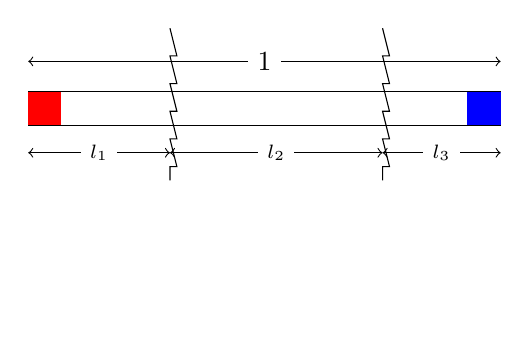
\begin{tikzpicture}
\draw (0,0) -- ++(6,0) -- ++(0,12pt) -- ++(-6,0) -- cycle;
\fill[red] (0,0) rectangle +(12pt,12pt);
\fill[blue] (6,0) rectangle +(-12pt,12pt);
\draw[<->] (0,23pt) --
  node[fill=white] {$1$} ++(6,0);
\draw[decorate,decoration=saw] (1.8,35pt) -- +(0,-55pt);
\draw[decorate,decoration=saw] (4.5,35pt) -- +(0,-55pt);
\draw[<->] (0,-10pt) --
  node[fill=white] {$\scriptstyle l_1$} (1.8,-10pt);
\draw[<->] (1.8,-10pt) --
  node[fill=white] {$\scriptstyle l_2$} (4.5,-10pt);
\draw[<->] (4.5,-10pt) --
  node[fill=white] {$\scriptstyle l_3$} (6,-10pt);
\path (0,-1) rectangle +(2,-1.5);
\end{tikzpicture}
\caption{Breaking a rod into three pieces}\label{f.rod1}
\end{subfigure}
\hspace{3em}
\begin{subfigure}[b]{.4\textwidth}
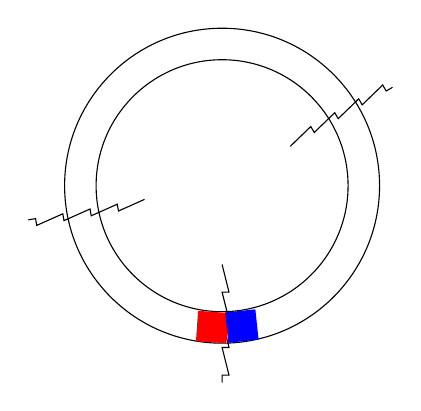
\begin{tikzpicture}
\draw (0,0) circle[radius=2];
\draw (0,0) circle[radius=1.6];
\draw[decorate,decoration=saw] (30:1) -- +(30:1.5);
\draw[decorate,decoration=saw] (190:1) -- +(190:1.5);
\draw[decorate,decoration=saw] (-90:1) -- +(-90:1.5);
\node[rotate=-4,fill=red,minimum width=11pt,minimum height=11pt]
  at (-94:1.8) {};
\node[rotate=6,fill=blue,minimum width=11pt,minimum height=11pt]
  at (-82:1.8) {};
\end{tikzpicture}
\caption{Breaking a ring into three pieces}\label{f.rod2}
\end{subfigure}
\end{center}
\end{figure}
\end{prob}

\solution{1}

The rods are not symmetric because the end pieces are different from the center piece. However, the ring is symmetric so the distributions of all three pieces must be uniform with expectation $1/3$. By choosing and coloring one of breaks as shown in Figure~\ref{f.rod2}, the problem is now the same as that of the rods so the distributions remain the same. Therefore the expectation of the lengths of the pieces is also $1/3$.

\solution{2}

Here is an elegant solution from \cite{stack-rods}.

Assume that the rod represents the line segment $(0,1)$. The rod is broken in two places which are represented as two uniform independent random variables $X,Y\in (0,1)$. Let us compute the probability $P(|X-Y|>a)$.

Table~\ref{t.rods} shows points $(x,y)$, where $x,y \in \{0.0, 0.1, 0.2, \ldots, 0.9\}$ and the decimal point is omitted. The values that appear in the table are $|X-Y|$. For $a=0.6$ the entries in the upper left corner $(0,6)$--$(6,9)$ and above, and the entries in the lower right corner $(6,0)$--$(9,6)$ and below, are those outcomes that define $P(|X-Y|>a)$:
\[
P(|X-Y|>a)=2\cdot \frac{1}{2}(1-a)(1-a)=(1-a)^2\,.
\]
For $a=0.6$, $P(|X-Y|>0.6)=(0.4)^2=0.16$.

\begin{table}[bt]
\[
\begin{array}{c}
\quad\\\\\\
a\\\\
\quad\\
y\\
\quad\\\quad\\\quad\\\quad
\end{array}
\begin{array}{|c|cccccccccc|}
\multicolumn{11}{l}{\qquad \qquad \qquad a}\\
\hline
9& 9 & 8 & 7 & 6 & 5 & 4 & 3 & 2 & 1 & 0  \\
8& 8 & 7 & 6 & 5 & 4 & 3 & 2 & 1 & 0 & 1  \\
7& 7 & 6 & 5 & 4 & 3 & 2 & 1 & 0 & 1 & 2  \\
6& 6 & 5 & 4 & 3 & 2 & 1 & 0 & 1 & 2 & 3  \\
5& 5 & 4 & 3 & 2 & 1 & 0 & 1 & 2 & 3 & 4  \\
4& 4 & 3 & 2 & 1 & 0 & 1 & 2 & 3 & 4 & 5  \\
3& 3 & 2 & 1 & 0 & 1 & 2 & 3 & 4 & 5 & 6  \\
2& 2 & 1 & 0 & 1 & 2 & 3 & 4 & 5 & 6 & 7  \\
1& 1 & 0 & 1 & 2 & 3 & 4 & 5 & 6 & 7 & 8  \\
0& 0 & 1 & 2 & 3 & 4 & 5 & 6 & 7 & 8 & 9  \\
\hline
&0 & 1 & 2 & 3 & 4 & 5 & 6 & 7 & 8 & 9  \\
\hline
\multicolumn{11}{c}{\quad \quad x\quad\quad\quad a}
\end{array}
\begin{array}{c}
\\\\\\
a\\\\
\end{array}
\]
\caption{Distribution of breaks on $(0,1)\times (0,1)$}\label{t.rods}
\end{table}

Taking the complement gives:
\[
P(|X-Y|<a)=1-(1-a)^2\,.
\]
This is the cumulative probability distribution (CPD) for the interval $(0,1)$. The probability density function (PDF) can be obtained by differentiating the CDP:
\[
P(|X-Y|=a)= \frac{d}{da}P(|X-Y|<a) =
  \frac{d}{da}(1-(1-a)^2)=2(1-a)\,.
\]
The expectation is the integral of the PDF multiplied by the value:
\[
E(|X-Y|)= \int_{0}^{1} a\cdot2(1-a)\, da=
  2\left.\left(\frac{a^2}{2}-\frac{a^3}{3}\right)\right|_0^1=\frac{1}{3}\,.
\]

\textbf{Simulation}
\begin{verbatim}
Expectation of length of right piece = 0.3333
Average length of right piece        = 0.3359
\end{verbatim}

%%%%%%%%%%%%%%%%%%%%%%%%%%%%%%%%%%%%%%%%%%%%%%%%%%%%%%%%%%%%%

\begin{prob}{The first ace}
Deal cards from a well-shuffled deck of cards until an ace appears. What is the expectation of the number of cards that must be dealt?

\textbf{Hint:} Consider the deck of cards without the aces to be laid out in a line.
\end{prob}

\solution{}

The cards form a ``rod'' of length $48$ which is ``broken'' by the $4$ aces into $5$ ``pieces.'' The solution of Problem~39 applies and the expectation of the length of a piece is $48/5=9.6$.

\textbf{Simulation}
\begin{verbatim}
Expectation of first ace = 9.6000
Average first ace        = 9.5805
\end{verbatim}

%%%%%%%%%%%%%%%%%%%%%%%%%%%%%%%%%%%%%%%%%%%%%%%%%%%%%%%%%%%%%

